\documentclass{article}
\usepackage[utf8]{inputenc}
\usepackage[margin=3cm]{geometry}
\title{CSEN 901: Introduction to Artificial Intelligence \\Project 1: Water Sort}
\author{Project Report \vspace{24pt} \\ Abdelrahman Aboelkehir, Hossain Ghoraba, \\ Mahmoud Aboelenein, Omar Hesham}
\date{18.10.2024}


\usepackage{natbib}
\usepackage{graphicx}
\usepackage{dirtree}
\usepackage{algorithm}
\usepackage{algpseudocode}
\usepackage{hyperref}


\begin{document}

\maketitle

\section{Introduction}
This project is the implementation of a search agent to solve the water sort puzzle. You can find a description of the water sort puzzle in the document titled \textbf{Project Description.pdf}. The agent is implemented in Java. The search the agent performs does not prune any branches early, nor does it perform any checks for whether the current node can or can not lead to a solution. A branch in the search is terminated only when there are no more possible nodes to expand from the leaf of that branch (in this probelm, this means there are no possible pour combinations to apply to the current state). The search terminates when either \textbf{a.} A node selected for expansion is identified as a goal state, or \textbf{b.} No more nodes on the search frontier can be expanded.


\section{Program Running Cycle}

For the water sort problem, running begins in the \texttt{WaterSortSearch} class. The class has a method \texttt{solve} that takes as an input a String \texttt{initialState}, which contains the initial configuration of the bottles and the layers within them, as well as the number of bottles and their capacities, encoded in a specified string format. It also takes a \texttt{strategy} specifying the search algorithm to use, and a boolean \texttt{visualize} that enables or disables printing various information about the run to the console. From there, the initial state is parsed into our \texttt{WaterSortState} structure using a parsing method in \texttt{WaterSortUtils}, a new \texttt{WaterSortProblem} is created using the initial state and the search strategy, and \texttt{executeSearchStrategy(WaterSortProblem waterSortProblem, String strategy, boolean visualize)}. \\

\texttt{executeSearchStrategy()} is a method in the \texttt{SearchStrategy} class that:

\begin{enumerate}
\item Gets the appropriate queuing function for the search algorithm based on the strategy
\item runs the corresponding \texttt{Search()} method, which itself just runs \texttt{generalSearch()} in the \texttt{GenericSearch} class.
\end{enumerate}

For example, here is the method for Breadth-First search: 
\begin{verbatim}
  public static Node BreadthFirstSearch(Problem problem,boolean visualize) throws 
  CloneNotSupportedException {
    return GenericSearch.generalSearch(problem, new EnqueueAtEnd(), visualize);
  }
\end{verbatim}

The return of this method is the node corresponding to a solution state (or \texttt{null}, if no solution is found).

\section{Project Hierarchy}

Here is a hierarchy of all the project files:

\dirtree{%
.1 src.
.2 code.
.3 generic.
.4 QueuingFunctions.
.5 QueuingFunction <<Interface>>.
.5 AStar1QueuingFunctions.
.6 AStar2QueuingFunction.
.6 EnqueueAtEnd.
.6 EnqueueAtFront.
.6 EnqueueAtFrontWithDepthLimit.
.6 GREEDY1QueuingFunction.
.6 GREEDY2QueuingFunction.
.5 FixedSizeStack.
.5 Operator <<Interface>>.
.5 OperatorResult.
.5 Problem.
.5 SearchState.
.6 OrderedInsert.
.4 utils.
.5 ConditionalPrintStream.
.5 Methods.
.5 WaterSortUtils.
.4 watersort.
.5 Bottle.
.5 Color.
.5 LayerGroup.
.5 Pour.
.5 WaterSortProblem.
.5 WaterSortState.
.5 WaterSortUtils.
.4 GenericSearch.
.4 Node.
.4 WaterSortSearch.
.2 tests.
.3 PublicTests.
}

\newpage

\begin{figure}[t]
\section{Class Diagram}
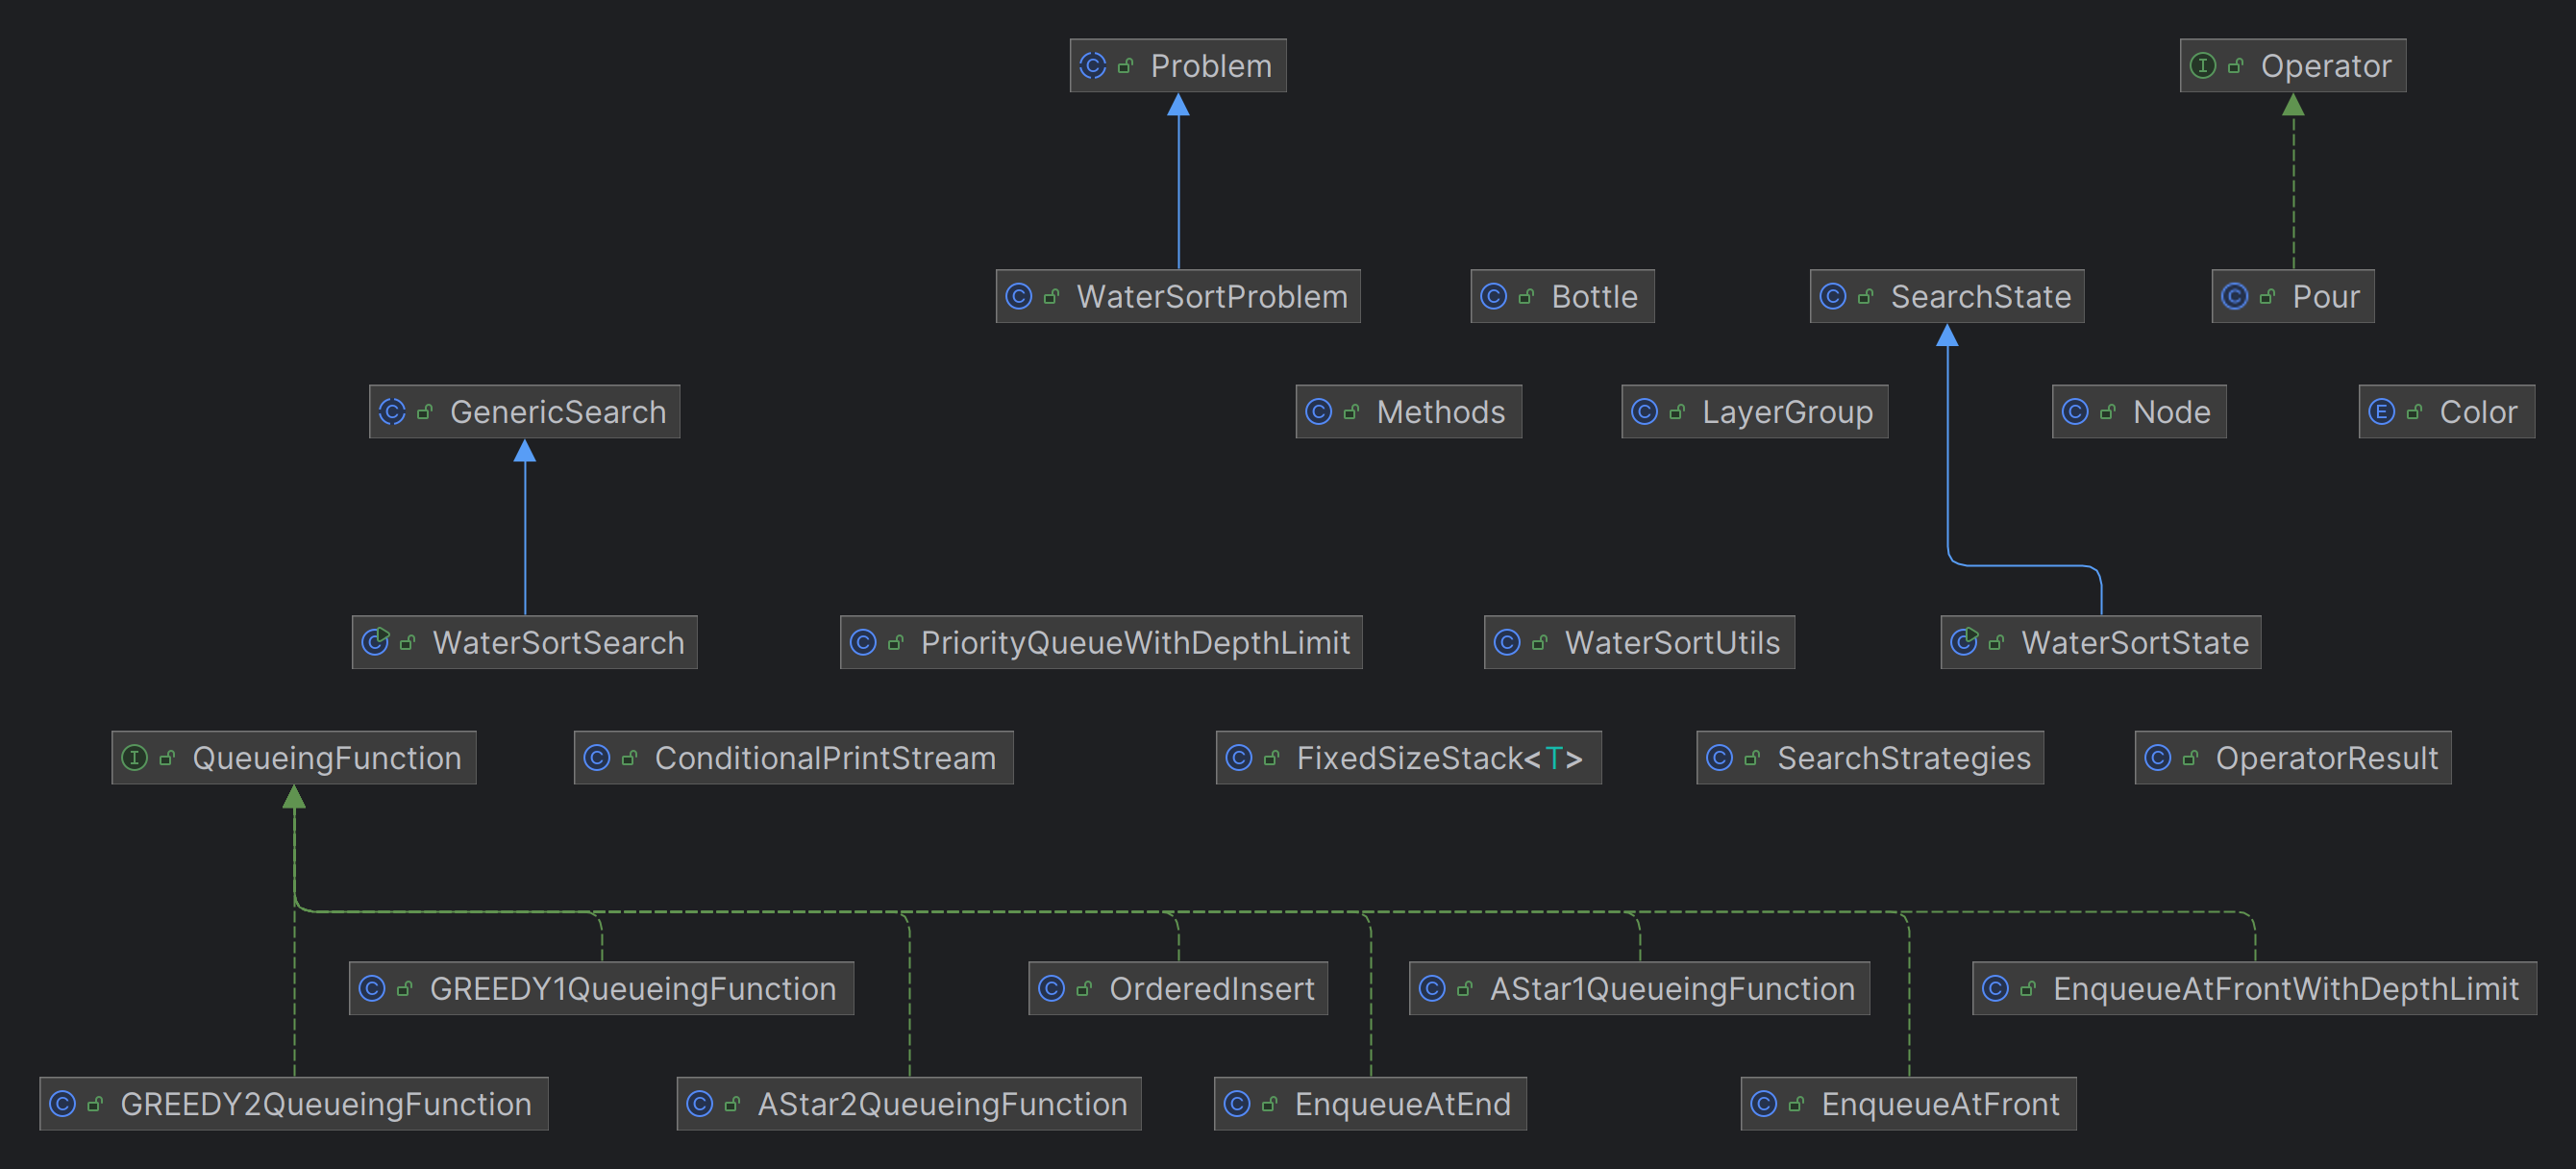
\includegraphics[scale=0.18]{Class Diagram.png}
\caption{Class Diagram}
\end{figure}

\section{Implementation of the Search Algorithms}

Our implementation for all search algorithms closely follows the description of the \textsl{GeneralSearch} algorithm outlined in lecture 2 of the course: 


\begin{algorithm}
\caption{GENERAL-SEARCH(problem, QING-FUN)}
\begin{algorithmic}[1]
    \State \textbf{return} a solution, or failure
    \State $nodes \gets \texttt{MAKE\_Q}(\texttt{MAKE\_NODE}(\texttt{INIT\_STATE}(problem)))$
    \While{true}
        \If{$nodes$ is empty}
            \State \textbf{return} failure
        \EndIf
        \State $node \gets \texttt{REMOVE\_FRONT}(nodes)$
        \If{$\texttt{GOAL\_TEST}(problem)(\texttt{STATE}(node))$}
            \State \textbf{return} node
        \EndIf
        \State $nodes \gets \texttt{QING\_FUN}(nodes, \texttt{EXPAND}(node, \texttt{OPER}(problem)))$
    \EndWhile
\end{algorithmic}
\end{algorithm}

All the algorithms use a Java \texttt{PriorityQueue} as their queue. The \texttt{PriorityQueue} in Java orders objects based on a given \texttt{Comparator}. The classes in the \texttt{QueueingFunctions} package create and return a \texttt{PriorityQueue} with the appropriate \texttt{Comparator}, which will then be used to hold and order all the nodes during the search. \\

\newpage

For example, here is the queuing function for Breadth-First Search: 

\begin{verbatim}
public class EnqueueAtEnd implements QueuingFunction {
  @Override
  public PriorityQueue<Node> apply() {
    return new PriorityQueue<>(Comparator.comparingInt(Node::getDepth));
  }
}
\end{verbatim}

In this case, a \texttt{PriorityQueue} is created using a comparator that says to order the nodes by depth in ascending order. Consequently, all the nodes in this queue will be ordered in ascending order of depth. \\

Here is a comprehensive list of the way by which the \texttt{PriorityQueue} orders nodes within it for every search algorithm we have implemented:

\begin{enumerate}
\item Breadth-First Search (BFS): Depth (ascending, i.e from \textit{shallowest} to \textit{deepest})
\item Depth-First Search (DFS): Depth (descending, i.e from \textit{deepest} to \textit{shallowest})
\item Iterative Deepening Depth-First Search (IDS): Same as DFS
\item Uniform-Cost Search (UCS): Path cost from the root to the node \texttt{(f(n) = g(n))}(ascending)
\item Greedy Best-First Search: The value of the heuristic function \texttt{(f(n) = h(n))}(we have two \textbf{admissible} heuristics we can use)
\item A* Search: The value of the path from the root plus the heuristic value for the current node (\texttt{f(n) = g(n) + h(n)})
\end{enumerate}

\newpage

Here is the main body of how searching is done (in the \texttt{GenericSearch} class):
\begin{verbatim}
public static Node generalSearch(Problem problem, QueuingFunction queuingFunction, boolean visualize)
            throws CloneNotSupportedException {
        nodesExpanded = 0;
        int nodesVisited = 0;
        Node solutionNode = null;
        expandedStates.clear();
        candidateSolutions.clear();

        Node initialNode = makeNode(problem.getInitialState());
        PriorityQueue<Node> nodes = queuingFunction.apply();
        nodes.add(initialNode);

        while (!nodes.isEmpty()) {
            Node currentNode = removeFront(nodes);
            currentNode.setOrderOfVisiting(nodesVisited++);
            if (problem.goalTestFn(currentNode)) {
                solutionNode = currentNode;
                break;
            }
            List<Node> expandedNodes = expand(currentNode, problem.getOperators(), problem);
            nodes.addAll(expandedNodes);
        }

        return solutionNode;
    }
\end{verbatim}

\subsubsection{Goal Test}
One important thing to mention is that the goal test is applied to a node first when it is selected for expansion, not when it is created. This has the unfortunate side-effect of increasing the time complexity of DFS from $O(b^{d})$ to $O(b^{d+1})$, because an extra level (at least in the worst case) will be created beyond the goal node before the goal node is selected for expansion and discovered to be a goal, as well as perhaps increasing the time complexity of the rest of the search algorithms (by a factor I am not entirely sure about), but has the fortunate side-effect of making UCS optimal (if the goal test was applied to a node when it is first created, UCS would not be optimal). If you are curious, you can find a small discussion of why this may be the case in Russel \& Norvig, section 3.4.2

\subsection{Eliminating Repeated States}

One important feature of any search algorithm is to minimize or eliminate repeated states that appear during the search. There are various degrees to which this can be done, each with its time and space efficiency trade-offs. We have chosen to go with the most extreme degree, which is to keep track of \textit{all} visited states during the search.
\subsection{Heuristic Functions}

We have mentioned earlier that we have two heuristic functions available for use. In this section, we will examine those two heuristic functions and argue why they may be admissible. \\

\textbf{Heuristic 1:} The number of bottles where the layers are not all the same color. \\

It is easy to show that this heuristic is admissible. For any state not to be a goal state, there must be at least 1 bottle where all the layers are not the same color. To make this state a goal state, you must pour at least 1 layer from one bottle to another. Therefore, this heuristic can never overestimate the cost (which is the number of layers poured) of the solution. \\


\textbf{Heuristic 2:} The difference between the current filled capacity of the bottle and the highest number of layers with the same color, all added up together.

For example, consider the following state with 3 bottles: \texttt{[e,e,r,g,r], [e,b,r,b,b,y], [e,e,e,e,e]}. The value of the heuristic function for this state will be: $(3 - 2) + (5 - 3) + (0) = 3$ \\

It is also not too difficult to show that this heuristic is admissible. If the node is a goal state (either all the bottles are empty, or all the bottles have layers of the same color), its value is 0. For a state that is only one layer away from a goal state, such as \texttt{[y,y,y,y,y], [e,g,b,b,b], [e,g,g,g,g]}, the value of the heuristic is $(0) + (1) + (0) = 1$. And this is in the "best-case" scenario where the layer to be poured is directly on top. If the layer(s) was/were anywhere other than on top, it would certainly take more than 1 pour operation to reach a goal state. Notice that we only calculate the difference between the filled capacity of the bottle and the number of the most repeated color layer. \\

The value of this heuristic for an empty bottle is therefore 0 (current capacity: 0 - number of most repeated color: 0, = 0.)



\subsection{Implementation of Iterative-Deepening Search}

Iterative-Deepening Search is special in that it is the only search algorithm that works differently from the remaining search algorithms. For the remaining search algorithms, nodes are simply added to the \texttt{PriorityQueue}, removed from the front of the queue, and expanded, until either the queue is empty (there are no more nodes left to expand), or a solution node has been found. IDS works differently in that it is the only search algorithm we have implemented that searches the whole tree from the root node more than once.

\begin{verbatim}
  public static Node IterativeDeepeningSearch(Problem problem, boolean visualize){
    int infinity  = Integer.MAX_VALUE;

    for(int depth = 0; depth < infinity; depth++){
      Node solution = DepthLimitedSearch(problem, depth, visualize);
      if(solution != null) {
        return solution;
      }
    }

    return null;
  }
\end{verbatim}

Our method for IDS runs DLS up to "infinity" (in Java, \texttt{Integer.MAX\_VALUE} is equal to 2,147,483,647 which we will assume is good enough for our purposes.) up to the specified \texttt{depth}, staring from 0 and incrementing the depth by 1 every iteration. Every time \texttt{DepthLimitedSearch} is called, it starts a new search problem, unrelated to the search in the previous iteration. 

\newpage

\texttt{LimitedDepthSearch} is just DFS that runs up to a specified depth limit. 

\begin{verbatim}
public static Node LimitedDepthSearch(Problem problem, int depth, boolean visualize) 
throws CloneNotSupportedException {
    return GenericSearch.generalSearch(problem, new EnqueueAtFrontWithDepthLimit(depth), visualize);
  }
\end{verbatim}

Its queuing function \texttt{EnqueueAtFrontWithDepthLimit} uses a custom data type that is a priority queue that only allows the addition of elements within a specified depth limit.


\begin{verbatim}
public class EnqueueAtFrontWithDepthLimit implements QueuingFunction {
  public int depthLimit;

  public EnqueueAtFrontWithDepthLimit(int depthLimit){
    this.depthLimit = depthLimit;
  }

  @Override
  public PriorityQueue<Node> apply() {
    return new PriorityQueueWithDepthLimit(Comparator.comparingInt(Node::getDepth).reversed(), depthLimit);
  }
}

\end{verbatim}

And here is how \texttt{PriorityQueueWithDepthLimit} is defined:

\begin{verbatim}
public class PriorityQueueWithDepthLimit extends PriorityQueue<Node> {
  private final int depthLimit;

  public PriorityQueueWithDepthLimit(int depthLimit) {
    super(); // Call to the default PriorityQueue constructor
    this.depthLimit = depthLimit;

  @Override
  public boolean addAll(Collection<? extends Node> nodes) {
    boolean modified = false;
    for (Node node : nodes) {
      if (node.getDepth() <= depthLimit) {
        modified |= super.add(node); // Add nodes only if within the depth limit
      }
    }
    return modified;
  }
}

  NOTE: Some code has been trimmed from this class for simplicity. 
  You can view the full code in the corresponding class file in the project.
\end{verbatim}

\newpage

\section{Comparison between the Search Algorithms}

In this section, we compare the completeness, optimality, and performance of the different search algorithms implemented in terms of RAM usage, CPU utilization, and the number of expanded nodes. We will also comment on the differences in RAM usage, CPU utilization, and expanded nodes between the search strategies.

\subsection{Completeness and Optimality}
\begin{itemize}
    \item \textbf{Breadth-First Search (BFS)}: BFS is complete assuming the branching factor is finite, and is optimal if the cost is a monotnoically nondecreasing function of the depth (i.e the cost at depth $d+1$ is equal to or higher than the cost at level $d$, and the cost increases in the direction of enqueuing (in our case, from left to right.) \\
    
    For the water sort problem, since there is a finite number of operators, the branching factor is finite, and therefore it is complete. Since all the operators have a positive cost (namely the only operator, \texttt{Pour}), the first condition for optimality holds. However, the cost does not necessarily increase as we go from left to right, because it depends on how many layers every operator will pour, depending on the state. Because of this, DFS is \textbf{complete} but \textbf{not optimal} for the water sort problem.

    \item \textbf{Depth-First Search (DFS)}: DFS is generally not complete, and it is not optimal. DFS explores as deep as possible before backtracking, making it prone to getting stuck in deep branches if no solution exists within the depth limit.

    \item \textbf{Iterative Deepening Search (IDS)}: IDS is complete, but generally not optimal. For the water sort problem, it is complete but not optimal for a similar reason to DFS.

    \item \textbf{Uniform-Cost Search (UCS)}: UCS is both complete and optimal for any search problem. Therefore, it is both complete and optimal for the water sort problem.

    \item \textbf{Greedy Best-First Search}: Greedy search is neither complete nor optimal. It chooses nodes based solely on the heuristic value, which can lead to suboptimal solutions or failure if the heuristic is misleading.

    \item \textbf{A* Search}: A* is both complete and optimal when using an admissible heuristic. In fact, it is also optimally efficient, where no other optimal search strategy will expand less nodes than A*. Since the two heuristics we are using for the water sort problem in this project are admissible (as we have already argued), A* is optimal for the water sort problem.
\end{itemize}

\subsection{Performance Metrics (RAM Usage, CPU Utilization, Number of Expanded Nodes)}

We've used the problem with the following initial state as our test case:
\begin{figure}[ht]
    \centering
    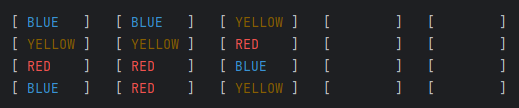
\includegraphics[width=0.5\textwidth]{TestCase1.png}
    \caption{Initial State}
    \label{fig:testcase1}
\end{figure}

We ran the following test case on all of the aforementioned algorithms and recorded the average results. The results were produced on a machine running 16 gigabytes of RAM and an Intel i7-8700 CPU.

\begin{table}[H]
    \centering
    \begin{tabular}{|l|c|c|c|c|c|}
        \hline
        \textbf{Algorithm} & \textbf{Memory Usage (RAM)} & \textbf{CPU Utilization} & \textbf{Number of Expanded Nodes} \\ \hline
        \textbf{BFS} & 4548 KB & 8.31\% & 789 \\ \hline
        \textbf{DFS} & 1106 KB & 7.89\% & 44 \\ \hline
        \textbf{IDS} & 5566 KB & 32.55\% & 1306 \\ \hline
        \textbf{UCS} & 3571 KB & 7.44\% & 676 \\ \hline
        \textbf{Greedy} & 491 KB & 5.92\% & 35 \\ \hline
        \textbf{A*} & 617 KB & 4.82\% & 58 \\ \hline
    \end{tabular}
    \caption{Comparison of Search Algorithms}
\end{table}

Note that the IDS results were obtained by aggregating the results from the iterations of Depth-Limited Search.

\subsection{Comparison Notes}

1. \textbf{Memory Usage (RAM)}:
\begin{itemize}
    \item \textbf{Best:} \textbf{Greedy Search} utilizes the least memory at \textbf{491 KB}, indicating a low memory footprint.
    \item \textbf{Worst:} \textbf{IDS (Iterative Deepening Search)} has the highest memory usage at \textbf{5566 KB}. This is because although it reduces the depth of recursion, it does so at the cost of significantly higher memory consumption.
\end{itemize}
2. \textbf{CPU Utilization}:
\begin{itemize}
    \item \textbf{Best:} \textbf{A*} shows the lowest CPU utilization at \textbf{4.82\%}, which could be attributed to its nature of taking into consideration the previous path cost and the future cost of the heuristic.
    \item \textbf{Worst:} \textbf{IDS} has the highest CPU utilization at \textbf{32.55\%}, due to the iterative deepening process which incurs a higher computational overhead.
\end{itemize}
3. \textbf{Number of Expanded Nodes}:
\begin{itemize}
    \item \textbf{Best:} \textbf{Greedy Search} also excels here with the fewest expanded nodes, only \textbf{35}, indicating that a well-designed heuristic in this case could result in good performance of greedy.
    \item \textbf{Worst:} \textbf{IDS} has the most expanded nodes at \textbf{1306}, consistent with its high memory and CPU usage.
\end{itemize}

\newpage

\section{Using the Agent to Implement and Solve Another Search Problem}

The primary goal of this project was to implement a search agent to solve the water sort puzzle, but another goal was also to have this agent be able to solve any generic search problem that the user defines. If you would like to use our agent to define and solve your own search problem, you have to do the following: 

\begin{enumerate}
\item Define a class for your problem that extends the \texttt{Problem} class
\item Define the operators for your problem. Each operator should be a class that implements the \texttt{Operator} interface.
\item If you would like to use another queuing function than the ones already defined (i.e you would like to use some other search algorithm than the 6 we have), define a queuing function for your problem. Your queuing function should implement the \texttt{QueuingFunction} interface.

\begin{itemize}
\item If you chose to define a new search strategy, go to the \texttt{SearchStrategy} class, give your new search strategy a \texttt{String} name, and add it to the switch case in the \texttt{executeSearchStrategy()} method.
\end{itemize}

\item Create a search class for your problem that extends the \texttt{GenericSearch} class. In this class, you will initialize an instance of your problem, the priority queue by using the queuing function, and call \texttt{executeSearchStrategy()}
\end{enumerate}

There is currently an unfortunate limitation regarding how heuristic functions are implemented. Because of this, if you would like to use greedy best-first search or A* search for your problem, you will not be able to use the provided ones. You will have to define new \texttt{QueueingFunction}s for them that order the nodes by \texttt{yourProblem.getHeuristicN()} in the case of greedy best-first and \texttt{Node.getPathCost()} + \texttt{yourProblem.getHeuristicN(Node node)} in the case of A* search, and implement any number of heuristic functions you would like in the class of your problem that you were asked to implement in item number \textbf{1}. You will need a \texttt{QueueingFunction} for every heuristic function you implement, unless you would like to order a single queue by the combination of more than one heuristic at the same time (e.g ordering by \texttt{getHeuristic1() + getHeuristic2()})

\section{References}
The main references we used to implement our project were: 

\begin{itemize}

\item The lecture slides of the CSEN 901: Introduction to Artificial Intelligence course taught at the GUC by Dr. Nourhan Ehab
\item Russell, S.J. and Norvig, P. (2016) Artificial Intelligence: A Modern Approach
\item The Java JDK 18 documentation (\url{https://docs.oracle.com/en/java/javase/18/})
\end{itemize}

We have not made use of any code from any external libraries. We have only made use of classes available in the java standard libraries.

\end{document}